\chapter{Introducción}

\section{Motivación}

En un mundo interconectado los ciberataques son uno de los mayores problemas para muchas organizaciones. Las organizaciones cada vez invierten más recursos en la detección de ataques informáticos, pero debido al amplio espectro de los mismos todavía tenemos serias dificultades para prevenirlos.

\bigskip
Las pérdidas en la economía mundial causadas por el cibercrimen y el ciberespionaje se estiman en cientos de miles de millones de dólares\cite{herrero_cibercrimen_2015}. Según un estudio del Instituto de Investigación Interregional de Crimen y Justicia de las Naciones Unidas (UNICRI por sus siglas en inglés), el cibercrimen es una de las principales amenazas para la economía mundial pasando el coste asociado al cibercrimen de 400.000 millones de Dólares en 2014\cite{zappa_cybercrime:_2014} a alcanzar, según la Interpol, una estimacionón de 750.000 millones de Euros sólo en Europa\cite{gil_cuanto_2018}.

\bigskip
Las pérdidas estimadas causadas por actividades cibernéticas maliciosas están dentro de los siguientes criterios\cite{armin_2020_2015}:

\begin{itemize}
  \item Robo de propiedad intelectual e información comercial confidencial.
  \item Robo de información sensible, incluida la posible manipulación del mercado.
  \item Coste de oportunidad que incluye interrupciones en el servicio, y una menor confianza en las actividades en línea.
  \item Pérdida causada por daños a la reputación de los negocios pirateados.
\end{itemize}

\bigskip
La forma mas común de realizar dichos ataques es haciendo uso de vulnerabilidades conocidas. Muchas de estas vulnerabilidades pueden ser causadas por una mala configuración o por una combinación inadecuada de parámetros. Asimismo, un servicio determinado puede tener prácticamente infinitas configuraciones posibles, siendo unas menos funcionales y/o vulnerables que otras.

\bigskip
La protección contra multitud de amenazas de seguridad informática puede ser implementada mediante una correcta configuración del software existente sin necesidad de invertir en costosas soluciones de seguridad.

\bigskip
Los algoritmos genéticos, que es una heurística de búsqueda, se pueden utilizan para descubrir configuraciones de computadora nuevas, seguras y diversas mediante el modelado de una determinada configuración como si fueran cromosomas y las distintas opciones de configuración individuales como si fueran genes\cite{gensch_evolving_2016}. La idea principal de los algoritmos genéticos es que mediante mutación, cruce y selección de dichos cromosomas obtendremos mejores configuraciones. Dichas mutaciones se incorporan al azar, lo que proporciona diversidad.

\bigskip
Para mejorar el mecanismo de protección contra los ciberataques, el atacante puede ser engañado por un cambio continuo en la configuración de un determinado servicio y en el caso de que el atacante sea capaz de descubrir vulnerabilidades en un programa específico el algoritmo genético habrá cambiado la configuración antes de que el atacante pueda definir un ataque en base a las vulnerabilidades descubiertas.

\bigskip
En nuestro caso concreto, los algoritmos genéticos nos proporcionarán una mejor seguridad a través de la diversidad\cite{crouse_improving_2012}.

\bigskip
Todo el código utilizado para la realización de este proyecto así como las diferentes herramientas tienen licencias de código abierto, tanto por motivación ideológica como por seguridad, ya que diversos estudios indican que el Software Libre es mucho mas seguro que el propietario\cite{clark_is_2009}.


\section{Definición del problema}

Un atacante suele comenzar su ataque realizando un reconocimiento previo. Luego planea su ataque de acuerdo con la información que encuentra, por lo tanto, un cambio periódico en la configuración es una ingeniosa forma de hacer que su esfuerzo de reconocimiento no sea efectivo y ayudaría a prevenir un ataque a un costo relativamente bajo.

\bigskip
La técnica del ``objetivo móvil'' o ``Moving Target Defense'' es aplicable incluso a elementos hardware como se ha visto en el diseño del procesador Morpheus que es capaz de cambiar su configuración interna cada 50 milisegundos\cite{gallagher_morpheus:_2019}.

\bigskip
En nuestro caso utilizaríamos un sistema de inteligencia artificial\cite{tribak_alisis_2012} para alterar la configuración de un servidor de forma regular saboteando así los esfuerzos de recopilación de información realizados por un posible atacante.

\bigskip
Las distintas configuraciones posibles van cambiando (mutando) mediante un algoritmo genético hasta alcanzar una solución óptima. Si dichas configuraciones óptimas son aplicadas de forma regular la información recopilada previamente por un posible atacante ya no es efectiva consiguiendo una capa de protección sencilla y económica a la vez que se optimiza la configuración del servicio\cite{john_evolutionary_2014}.

\bigskip
Es importante asegurarse de que las configuraciones generadas funcionen de una manera correcta, y es importante que dicha configuración sea segura. Es difícil encontrar una configuración segura debido a la gran cantidad de configuraciones para probar, y además de eso, es difícil encontrar la combinación entre las configuraciones que hace que los componentes sean seguros. Para solucionar este problema deberemos contar con una herramienta que nos pueda indicar el nivel de seguridad de una configuración determinada.


\section{Estructura del proyecto}

\bigskip
Antes de pasar a detalles más técnicos, me gustaría detallar el contenido de este proyecto:

\begin{itemize}
  \item En el \textit{capítulo 1} (\textbf{Introducción}) se encuentra una breve introducción a nuestra idea, así como las motivaciones que nos han llevado a realizarla.
  \item El \textit{capítulo 2} (\textbf{Objetivos}) define los objetivos que se quieren alcanzar con este proyecto.
  \item En el \textit{capítulo 3} (\textbf{Antecedentes}) se analiza el estado de arte actual, así como algunas de las tecnologías y paradigmas que utilizaremos en nuestro proyecto.
  \item En el \textit{capítulo 4} (\textbf{Metodología}) está la planificación y desarrollo de cada uno de los apartados del proyecto.
  \item En el \textit{capítulo 5} (\textbf{Resultados})se detallan todos los resultados obtenidos.
  \item En el \textit{capítulo 6} (\textbf{Conclusiones}) se pueden encontrar las conclusiones finales  así como las recomendaciones para futuros trabajos.

\end{itemize}

\bigskip
Para finalizar se incluye un anexo con el código fuente desarrollado y liberado bajo la licencia libre \cite{gplv3}. Dicho código fuente también se puede encontrar en la url \url{https://github.com/erseco/moving_target_defense}.



% %
% % Ejemplos de codigo LaTeX para uso futuro
% %

% \begin{figure}[h!]
% \centering
% 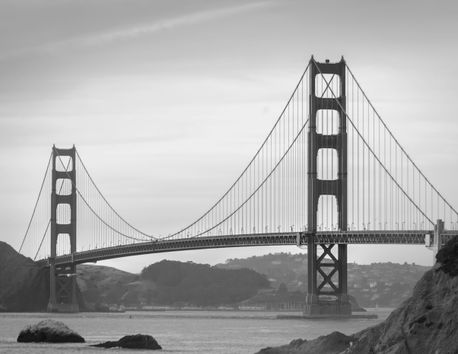
\includegraphics[width=1.0\textwidth]{../images/sample1}
% \caption{Sample Image 1}
% \label{fig:sample1}
% \end{figure}

% Esto es un texto con una nota\footnote{Ejemplo de nota al pie} al pie.

% Y esto es una ``Frase de alguien'' (\cite{john_evolutionary_2014}).

% \begin{itemize}
%   \item \textbf{1.} Texto de ejemplo
%   \item \textbf{2.} Texto de ejemplo
%   \item \textbf{3.} Texto de ejemplo
%   \item \textbf{4.} Texto de ejemplo

% \end{itemize}

% \begin{enumerate}
% 	\item Ejemplo 1.
% 	\item Ejemplo 2.
% \end{enumerate}

% \begin{lstlisting}[language=html]
% <!DOCTYPE html>
% <html lang="es-ES">
%   <head>
%     <meta charset="utf-8">
%     <title>Ejemplo de 2 párrafos</title>
%   </head>
%   <body>
%     <p>Esto es un párrafo.</p>
%     <p>Esto es otro párrafo.</p>
%   </body>
% </html>
% \end{lstlisting}

% Puedes verlo en \cite{merelo-guervos_comparison_2016}. Te recomiendo leer \cite{clark_is_2009, zhang_genetic_2009, schlenker_deceiving_2018, gensch_evolving_2016}.
